\subsection{QuizziPedia::Back-End::Config}
\subsubsection{Informazioni generali}
\label{QuizziPedia::Back-End::Config}
\begin{figure}
	\centering<
	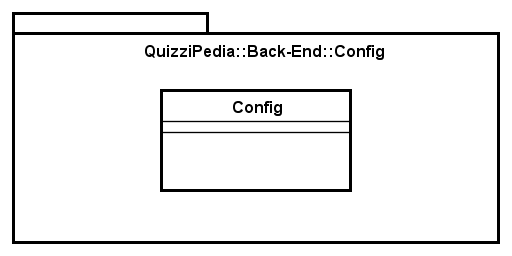
\includegraphics[scale=0.45]{UML/Package/QuizziPedia_Back-End_Config.png}
	\caption{QuizziPedia::Back-End::Config}
\end{figure}
	\begin{itemize}
		\item \textbf{Descrizione} \\
		Package contenente le copmonenti di configurazione del server.
		\item \textbf{Padre}: Back-End
		\item \textbf{Interazioni con altri componenti}:
			\begin{itemize}
				\item \texttt{App} \\
				Package contenente le componenti del server che implementano il \textit{pattern MVC\ped{G}}.
			\end{itemize}
	\end{itemize}
\subsubsection{Classi}
\paragraph{QuizziPedia::Back-End::Config::Config}
\label{QuizziPedia::Back-End::Config::Config}
\begin{figure}
	\centering
	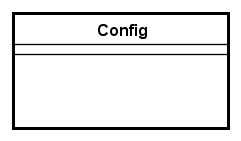
\includegraphics[scale=0.45]{UML/Classi/Back-End/QuizziPedia_Back-End_Config_Config.png}
	\caption{QuizziPedia::Back-End::Config::Config}
	\end{figure}
	\begin{itemize}
		\item \textbf{Descrizione} \\
		Questa classe gestisce la configurazione del server. \textit{Non sono stati modellati attributi e metodi di questa classe in quanto viene gestita da Express}
		\item \textbf{Utilizzo} \\
		Viene utilizzata per descrivere i parametri dell'applicazione. La classe \texttt{Server} utilizza oggetti di questo tipo per creare ed avviare l'istanza del server.
		\item \textbf{Relazioni con le altre classi}:
		 \begin{itemize}
		 	\item \textit{IN} \texttt{Server} \\
		 	Classe che avvia il server. Nello specifico apre una connessione al database tramite Mongoose, invoca il middleware\ped{G} Express\ped{G} passando un riferimento al database MongoDB\ped{G} come parametro in modo  che possa configurarsi con esso, invoca il middleware\ped{G} Passport\ped{G} ed infine si mette in ascolto su una determinata porta. E' il componente client del design pattern \textit{Chain of responsibility\ped{G}}. Utilizza i moduli Mongoose\ped{G}, Express\ped{G}, Passport\ped{G}.
		 \end{itemize}
	\end{itemize}
